% Options for packages loaded elsewhere
\PassOptionsToPackage{unicode}{hyperref}
\PassOptionsToPackage{hyphens}{url}
\PassOptionsToPackage{dvipsnames,svgnames,x11names}{xcolor}
%
\documentclass[
]{acmconf}
\usepackage{amsmath,amssymb}
\usepackage{lmodern}
\usepackage{iftex}
\ifPDFTeX
  \usepackage[T1]{fontenc}
  \usepackage[utf8]{inputenc}
  \usepackage{textcomp} % provide euro and other symbols
\else % if luatex or xetex
  \usepackage{unicode-math}
  \defaultfontfeatures{Scale=MatchLowercase}
  \defaultfontfeatures[\rmfamily]{Ligatures=TeX,Scale=1}
\fi
% Use upquote if available, for straight quotes in verbatim environments
\IfFileExists{upquote.sty}{\usepackage{upquote}}{}
\IfFileExists{microtype.sty}{% use microtype if available
  \usepackage[]{microtype}
  \UseMicrotypeSet[protrusion]{basicmath} % disable protrusion for tt fonts
}{}
\makeatletter
\@ifundefined{KOMAClassName}{% if non-KOMA class
  \IfFileExists{parskip.sty}{%
    \usepackage{parskip}
  }{% else
    \setlength{\parindent}{0pt}
    \setlength{\parskip}{6pt plus 2pt minus 1pt}}
}{% if KOMA class
  \KOMAoptions{parskip=half}}
\makeatother
\usepackage{xcolor}
\IfFileExists{xurl.sty}{\usepackage{xurl}}{} % add URL line breaks if available
\IfFileExists{bookmark.sty}{\usepackage{bookmark}}{\usepackage{hyperref}}
\hypersetup{
  pdftitle={Dynamics in Algorithmic Recourse},
  pdfauthor={Patrick Altmeyer},
  colorlinks=true,
  linkcolor={blue},
  filecolor={Maroon},
  citecolor={Blue},
  urlcolor={Blue},
  pdfcreator={LaTeX via pandoc}}
\urlstyle{same} % disable monospaced font for URLs
\setlength{\emergencystretch}{3em} % prevent overfull lines
\setcounter{secnumdepth}{5}
% Make \paragraph and \subparagraph free-standing
\ifx\paragraph\undefined\else
  \let\oldparagraph\paragraph
  \renewcommand{\paragraph}[1]{\oldparagraph{#1}\mbox{}}
\fi
\ifx\subparagraph\undefined\else
  \let\oldsubparagraph\subparagraph
  \renewcommand{\subparagraph}[1]{\oldsubparagraph{#1}\mbox{}}
\fi


\providecommand{\tightlist}{%
  \setlength{\itemsep}{0pt}\setlength{\parskip}{0pt}}\usepackage{longtable,booktabs,array}
\usepackage{calc} % for calculating minipage widths
% Correct order of tables after \paragraph or \subparagraph
\usepackage{etoolbox}
\makeatletter
\patchcmd\longtable{\par}{\if@noskipsec\mbox{}\fi\par}{}{}
\makeatother
% Allow footnotes in longtable head/foot
\IfFileExists{footnotehyper.sty}{\usepackage{footnotehyper}}{\usepackage{footnote}}
\makesavenoteenv{longtable}
\usepackage{graphicx}
\makeatletter
\def\maxwidth{\ifdim\Gin@nat@width>\linewidth\linewidth\else\Gin@nat@width\fi}
\def\maxheight{\ifdim\Gin@nat@height>\textheight\textheight\else\Gin@nat@height\fi}
\makeatother
% Scale images if necessary, so that they will not overflow the page
% margins by default, and it is still possible to overwrite the defaults
% using explicit options in \includegraphics[width, height, ...]{}
\setkeys{Gin}{width=\maxwidth,height=\maxheight,keepaspectratio}
% Set default figure placement to htbp
\makeatletter
\def\fps@figure{htbp}
\makeatother
\newlength{\cslhangindent}
\setlength{\cslhangindent}{1.5em}
\newlength{\csllabelwidth}
\setlength{\csllabelwidth}{3em}
\newlength{\cslentryspacingunit} % times entry-spacing
\setlength{\cslentryspacingunit}{\parskip}
\newenvironment{CSLReferences}[2] % #1 hanging-ident, #2 entry spacing
 {% don't indent paragraphs
  \setlength{\parindent}{0pt}
  % turn on hanging indent if param 1 is 1
  \ifodd #1
  \let\oldpar\par
  \def\par{\hangindent=\cslhangindent\oldpar}
  \fi
  % set entry spacing
  \setlength{\parskip}{#2\cslentryspacingunit}
 }%
 {}
\usepackage{calc}
\newcommand{\CSLBlock}[1]{#1\hfill\break}
\newcommand{\CSLLeftMargin}[1]{\parbox[t]{\csllabelwidth}{#1}}
\newcommand{\CSLRightInline}[1]{\parbox[t]{\linewidth - \csllabelwidth}{#1}\break}
\newcommand{\CSLIndent}[1]{\hspace{\cslhangindent}#1}

\ConferenceShortName{AIES '22}
\ConferenceName{Fifth AAAI/ACM Conference on Artificial Intelligence, Ethics, and Society}
\makeatletter
\makeatother
\makeatletter
\@ifpackageloaded{caption}{}{\usepackage{caption}}
\AtBeginDocument{%
\ifdefined\contentsname
  \renewcommand*\contentsname{Table of contents}
\else
  \newcommand\contentsname{Table of contents}
\fi
\ifdefined\listfigurename
  \renewcommand*\listfigurename{List of Figures}
\else
  \newcommand\listfigurename{List of Figures}
\fi
\ifdefined\listtablename
  \renewcommand*\listtablename{List of Tables}
\else
  \newcommand\listtablename{List of Tables}
\fi
\ifdefined\figurename
  \renewcommand*\figurename{Figure}
\else
  \newcommand\figurename{Figure}
\fi
\ifdefined\tablename
  \renewcommand*\tablename{Table}
\else
  \newcommand\tablename{Table}
\fi
}
\@ifpackageloaded{float}{}{\usepackage{float}}
\floatstyle{ruled}
\@ifundefined{c@chapter}{\newfloat{codelisting}{h}{lop}}{\newfloat{codelisting}{h}{lop}[chapter]}
\floatname{codelisting}{Listing}
\newcommand*\listoflistings{\listof{codelisting}{List of Listings}}
\makeatother
\makeatletter
\@ifpackageloaded{caption}{}{\usepackage{caption}}
\@ifpackageloaded{subcaption}{}{\usepackage{subcaption}}
\makeatother
\makeatletter
\@ifpackageloaded{tcolorbox}{}{\usepackage[many]{tcolorbox}}
\makeatother
\makeatletter
\@ifundefined{shadecolor}{\definecolor{shadecolor}{rgb}{.97, .97, .97}}
\makeatother
\makeatletter
\makeatother
\ifLuaTeX
  \usepackage{selnolig}  % disable illegal ligatures
\fi

\title{Dynamics in Algorithmic Recourse}
\author{Patrick Altmeyer}
\date{April 25, 2022}

\begin{document}
\maketitle

\ifdefined\Shaded\renewenvironment{Shaded}{\begin{tcolorbox}[interior hidden, borderline west={3pt}{0pt}{shadecolor}, sharp corners, frame hidden, boxrule=0pt, enhanced, breakable]}{\end{tcolorbox}}\fi

Recent advances in artificial intelligence (AI) have propelled its
adoption in domains outside of computer science including health care,
bioinformatics and genetics. In finance, economics and other social
sciences, applications of AI are still relatively limited.
Decision-making in these fields has traditionally been guided by
Generalized Linear Models (GLM), which are theoretically founded,
interpretable and often sufficient to model relationships between
variables. Model interpretability is crucial in the social sciences
context, because inference is typically at least as important as
predictive performance. Decision-makers in the social sciences are also
typically required to explain their decisions to human stakeholders:
central bankers, for example, are held accountable by the public for the
policies they decide on. It is therefore not surprising that
practitioners and academics in these fields are reluctant to adopt AI
technologies that ultimately cannot be trusted. Deep learning models,
for example, are generally considered as black boxes and therefore
difficult to apply in a context that demands explanations.

In my research I explore and develop methodologies that improve the
trustworthiness of AI. I would like to understand how we can unlock the
enormous potential of AI without sacrificing the human aspect of
decision-making in finance and economics. My work so far has focused
primarily on counterfactual explanations, algorithmic recourse and
probabilistic machine learning. Counterfactual explanations are
intuitive, largely model-agnostic and straight-forward to implement.
They are also intrinsically linked to the potential outcome framework
for causal inference and therefore should be somewhat familiar to social
scientists. Counterfactual explanations that involve realistic and
actionable changes can be used for the purpose of algorithmic recourse
to help individuals facing adverse decisions. Probabilistic machine
learning can be leveraged in this context and more generally facilitates
inference and interpretability. It is also closely related to Bayesian
statistics, which has played an important role in both finance and
economics for many years.

In the following (Section~\ref{sec-main}), I will first briefly present
one particular research question I have explored during the first months
of my PhD: how do counterfactual explanations handle dynamics? I will
also briefly present related projects I have worked on
(Section~\ref{sec-related}) and ideas for future projects
(Section~\ref{sec-future}).

\hypertarget{sec-main}{%
\section{Dynamics in Algorithmic Recourse}\label{sec-main}}

Existing work on counterfactual explanations and algorithmic recourse
has largely been limited to the following static setting: given some
classifier \(M: \mathcal{X} \mapsto \mathcal{Y}\) we are interested in
finding close (Wachter, Mittelstadt, and Russell 2017), actionable
(Ustun, Spangher, and Liu 2019), plausible Schut et al. (2021), sparse
(Schut et al. 2021), diverse (Mothilal, Sharma, and Tan 2020) and
ideally causally founded counterfactual explanations (Karimi, Schölkopf,
and Valera 2021) for some individual \(x\). The ability of
counterfactual explanations to handle dynamics like data and model
shifts remains a largely unexplored research challenge at this point
(Verma, Dickerson, and Hines 2020). Only one recent work considers the
implications of \textbf{exogenous} domain shifts on the validity of
recourse (Upadhyay, Joshi, and Lakkaraju 2021). The authors propose a
simple minimax objective, that minimizes the counterfactual loss
function for a maximal domain and model shift. They show that their
approach yields more robust counterfactuals than existing approaches. In
my project I investigate \textbf{endogenous} domain and model shifts,
i.e.~shifts that occur as algorithmic recourse is actually impemented by
a proportion of individuals. Preliminary findings indicate that
individuals who receive and implement algorithmic recourse end up
forming a distinct subgroup inside the target class, which may leave
them vulnerable to discrimination (Figure~\ref{fig-dynamics}). This is a
work-in-progress that I would like to present and discuss at AIES.

\begin{figure}

{\centering 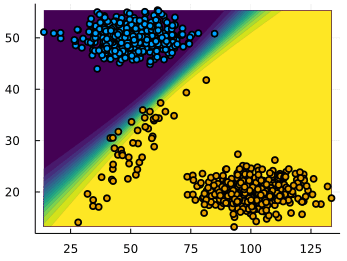
\includegraphics[width=2.60417in,height=\textheight]{www/dynamics.png}

}

\caption{\label{fig-dynamics}PLACEHOLDER: The dynamics of algorithmic
recourse.}

\end{figure}

\hypertarget{sec-related}{%
\section{Related Projects}\label{sec-related}}

Alongside my research I have developed open-source implementations
related to explainable AI.
\href{https://www.paltmeyer.com/CounterfactualExplanations.jl/stable/}{CounterfactualExplanations.jl}
is a Julia package that can be used to generate counterfactual
explanations for models developed and trained not only in Julia, but
also in other popular programming languages like Python and R. I have
recently submitted the package along with a companion paper as a
proposal for a main talk at \href{https://juliacon.org/2022/}{JuliaCon}.
\href{https://www.paltmeyer.com/BayesLaplace.jl/dev/}{BayesLaplace.jl}
is a small Julia package that can be used to recover Bayesian
representations of deep neural networks through Laplace approximation in
a post-hoc manner. It is inspired by a recent paper (Daxberger et al.
2021) and has also been submitted to JuliaCon. Finally,
\href{https://github.com/pat-alt/deepvars}{deepvars} is an R package
that implements an approach towards vector autoregression that leverages
deep learning. This was originally my master's thesis and later
presented at the NeurIPS 2021 MLECON workshop. I have also published
several blog posts on explainable AI and probabilisitic ML in an effort
to make my research accessible to a broad audience.

\hypertarget{sec-future}{%
\section{Future Projects}\label{sec-future}}

Data sets in finance and economics typically involve time series data.
Therefore, I am naturally interested in the application of explainable
AI to sequential data, an area which has so far not been explored
extensively. In the future, I want to work on counterfactual
explanations for time series models. I am also interested in seeing if
and how Laplace approximation can be used for Bayesian deep learning
with time series data. I hope that the findings from both of these
projects can ultimately be used to build complex but interpretable time
series models for classification and forecasting in finance and
economics. For example, I would like to leverage effortless Bayesian
deep learning to make our proposed Deep Vector Autoregression model
explainable.

\hypertarget{references}{%
\section*{References}\label{references}}
\addcontentsline{toc}{section}{References}

\hypertarget{refs}{}
\begin{CSLReferences}{1}{0}
\leavevmode\vadjust pre{\hypertarget{ref-antoran2020getting}{}}%
Antorán, Javier, Umang Bhatt, Tameem Adel, Adrian Weller, and José
Miguel Hernández-Lobato. 2020. {``Getting a Clue: A Method for
Explaining Uncertainty Estimates.''} \emph{arXiv Preprint
arXiv:2006.06848}.

\leavevmode\vadjust pre{\hypertarget{ref-daxberger2021laplace}{}}%
Daxberger, Erik, Agustinus Kristiadi, Alexander Immer, Runa Eschenhagen,
Matthias Bauer, and Philipp Hennig. 2021. {``Laplace Redux-Effortless
Bayesian Deep Learning.''} \emph{Advances in Neural Information
Processing Systems} 34.

\leavevmode\vadjust pre{\hypertarget{ref-joshi2019towards}{}}%
Joshi, Shalmali, Oluwasanmi Koyejo, Warut Vijitbenjaronk, Been Kim, and
Joydeep Ghosh. 2019. {``Towards Realistic Individual Recourse and
Actionable Explanations in Black-Box Decision Making Systems.''}
\emph{arXiv Preprint arXiv:1907.09615}.

\leavevmode\vadjust pre{\hypertarget{ref-karimi2021algorithmic}{}}%
Karimi, Amir-Hossein, Bernhard Schölkopf, and Isabel Valera. 2021.
{``Algorithmic Recourse: From Counterfactual Explanations to
Interventions.''} In \emph{Proceedings of the 2021 ACM Conference on
Fairness, Accountability, and Transparency}, 353--62.

\leavevmode\vadjust pre{\hypertarget{ref-mothilal2020explaining}{}}%
Mothilal, Ramaravind K, Amit Sharma, and Chenhao Tan. 2020.
{``Explaining Machine Learning Classifiers Through Diverse
Counterfactual Explanations.''} In \emph{Proceedings of the 2020
Conference on Fairness, Accountability, and Transparency}, 607--17.

\leavevmode\vadjust pre{\hypertarget{ref-schut2021generating}{}}%
Schut, Lisa, Oscar Key, Rory Mc Grath, Luca Costabello, Bogdan
Sacaleanu, Yarin Gal, et al. 2021. {``Generating Interpretable
Counterfactual Explanations by Implicit Minimisation of Epistemic and
Aleatoric Uncertainties.''} In \emph{International Conference on
Artificial Intelligence and Statistics}, 1756--64. PMLR.

\leavevmode\vadjust pre{\hypertarget{ref-upadhyay2021towards}{}}%
Upadhyay, Sohini, Shalmali Joshi, and Himabindu Lakkaraju. 2021.
{``Towards Robust and Reliable Algorithmic Recourse.''} \emph{arXiv
Preprint arXiv:2102.13620}.

\leavevmode\vadjust pre{\hypertarget{ref-ustun2019actionable}{}}%
Ustun, Berk, Alexander Spangher, and Yang Liu. 2019. {``Actionable
Recourse in Linear Classification.''} In \emph{Proceedings of the
Conference on Fairness, Accountability, and Transparency}, 10--19.

\leavevmode\vadjust pre{\hypertarget{ref-verma2020counterfactual}{}}%
Verma, Sahil, John Dickerson, and Keegan Hines. 2020. {``Counterfactual
Explanations for Machine Learning: A Review.''} \emph{arXiv Preprint
arXiv:2010.10596}.

\leavevmode\vadjust pre{\hypertarget{ref-wachter2017counterfactual}{}}%
Wachter, Sandra, Brent Mittelstadt, and Chris Russell. 2017.
{``Counterfactual Explanations Without Opening the Black Box: Automated
Decisions and the GDPR.''} \emph{Harv. JL \& Tech.} 31: 841.

\end{CSLReferences}



\end{document}
